\documentclass[10pt,reqno, final]{ctexart}
%\documentclass{ctexartutf8}
\topmargin=1cm \textwidth=14cm \textheight=21.5cm\oddsidemargin1.2cm\evensidemargin 1.2cm
\usepackage[ bookmarksnumbered, bookmarksopen, colorlinks, citecolor=blue, linkcolor=magenta, unicode]{hyperref}
\usepackage[notcite,notref]{showkeys}

\usepackage{url,hyperref,multirow}
\usepackage{color}
\usepackage{stmaryrd}
\usepackage{exscale}
\usepackage{setspace}
\usepackage{relsize}


\usepackage{epsfig,subfigure,amssymb,amsmath,version}
\usepackage{amssymb,version,graphicx,fancybox,mathrsfs,bm,pifont,booktabs}%,wrapfig}
\usepackage{cases}
\usepackage{epstopdf}

\usepackage{float}
\usepackage{graphicx}
%\usepackage{pythonhighlight}


\renewcommand{\theequation}{\thesection.\arabic{equation}}
\newtheorem{lemma}{引理}[section]
\newtheorem{theorem}{定理}[section]
\newtheorem{corollary}{推论}[section]
\newtheorem{proposition}{性质}[section]
\newtheorem{definition}{定义}[section]
\newtheorem{remark}{注}[section]
\newtheorem{example}{例}[section]

\begin{document}
\title{电磁场理论基础}
\author{张\quad 瑞}
\maketitle
\section{简介}
本文拟从电场与磁场的基本物理定律出发,推导出电磁场的Maxwell方程,再通过Maxwell方程得到电场和磁场在空间中的存在形式,即电磁波,而后研究电磁波在空间中传播的由简单到一般的各种模型。由于传播空间的无界性,在实际使用有限元计算的时候,需要应对无界区域,从而导出人工边界方法和完美匹配层 (PML)方法。

\section{Maxwell 方程的发展与推导及其物理含义}
\subsection{静电场}
\paragraph{场强矢量$\bm{E}$}在真空中放置一个点电荷,那么这个电荷会在空间中激发出电场,物理学中使用电场线来刻画电场的方向和大小,电场线从正电荷出发,指向负电荷,这便是场强的方向。而场强的大小是通过穿过单位面积的电场线的条数来定义的,即:
\begin{equation}\label{electricfield}
|\bm{E}|=\frac{N_e}{S},
\end{equation}
而穿过给定面积的曲面的电场线条数又叫做穿过这个曲面的\textbf{电通量},所以电场强度的\textbf{大小}又称为\textbf{电通量密度},见图 \ref{eandcoulumb} 左。
\paragraph{库仑力}位于坐标原点的点电荷$q$对位于$\bm{r}$处的试探电荷$Q$的电场力为:
\begin{equation}\label{coulombforce}
\bm{F}(\bm{r}) = \frac{1}{4\pi\varepsilon_0}\frac{Qq\bm{r}}{|\bm{r}|^3}.
\end{equation}
当然,在一般的文献中电荷量为$q$的点电荷在$\bm{r}$处的电场强度的定义是通过单位试探电荷在电场中所受到的库仑力来定义的,即:
\begin{equation}\label{columb}
\bm{E}(\bm{r})=\frac{1}{4\pi\varepsilon_0}\frac{q\bm{r}}{|\bm{r}|^3},
\end{equation}
其中,$\varepsilon_0$ 称为真空中的介电常数,见图 \ref{eandcoulumb} 右。值得注意的是不管有没有试探电荷的存在,点电荷在空间中激发的电场始终存在,只是没有了试探电荷那么库仑力为零。

\begin{figure}[htp]
	\centering
	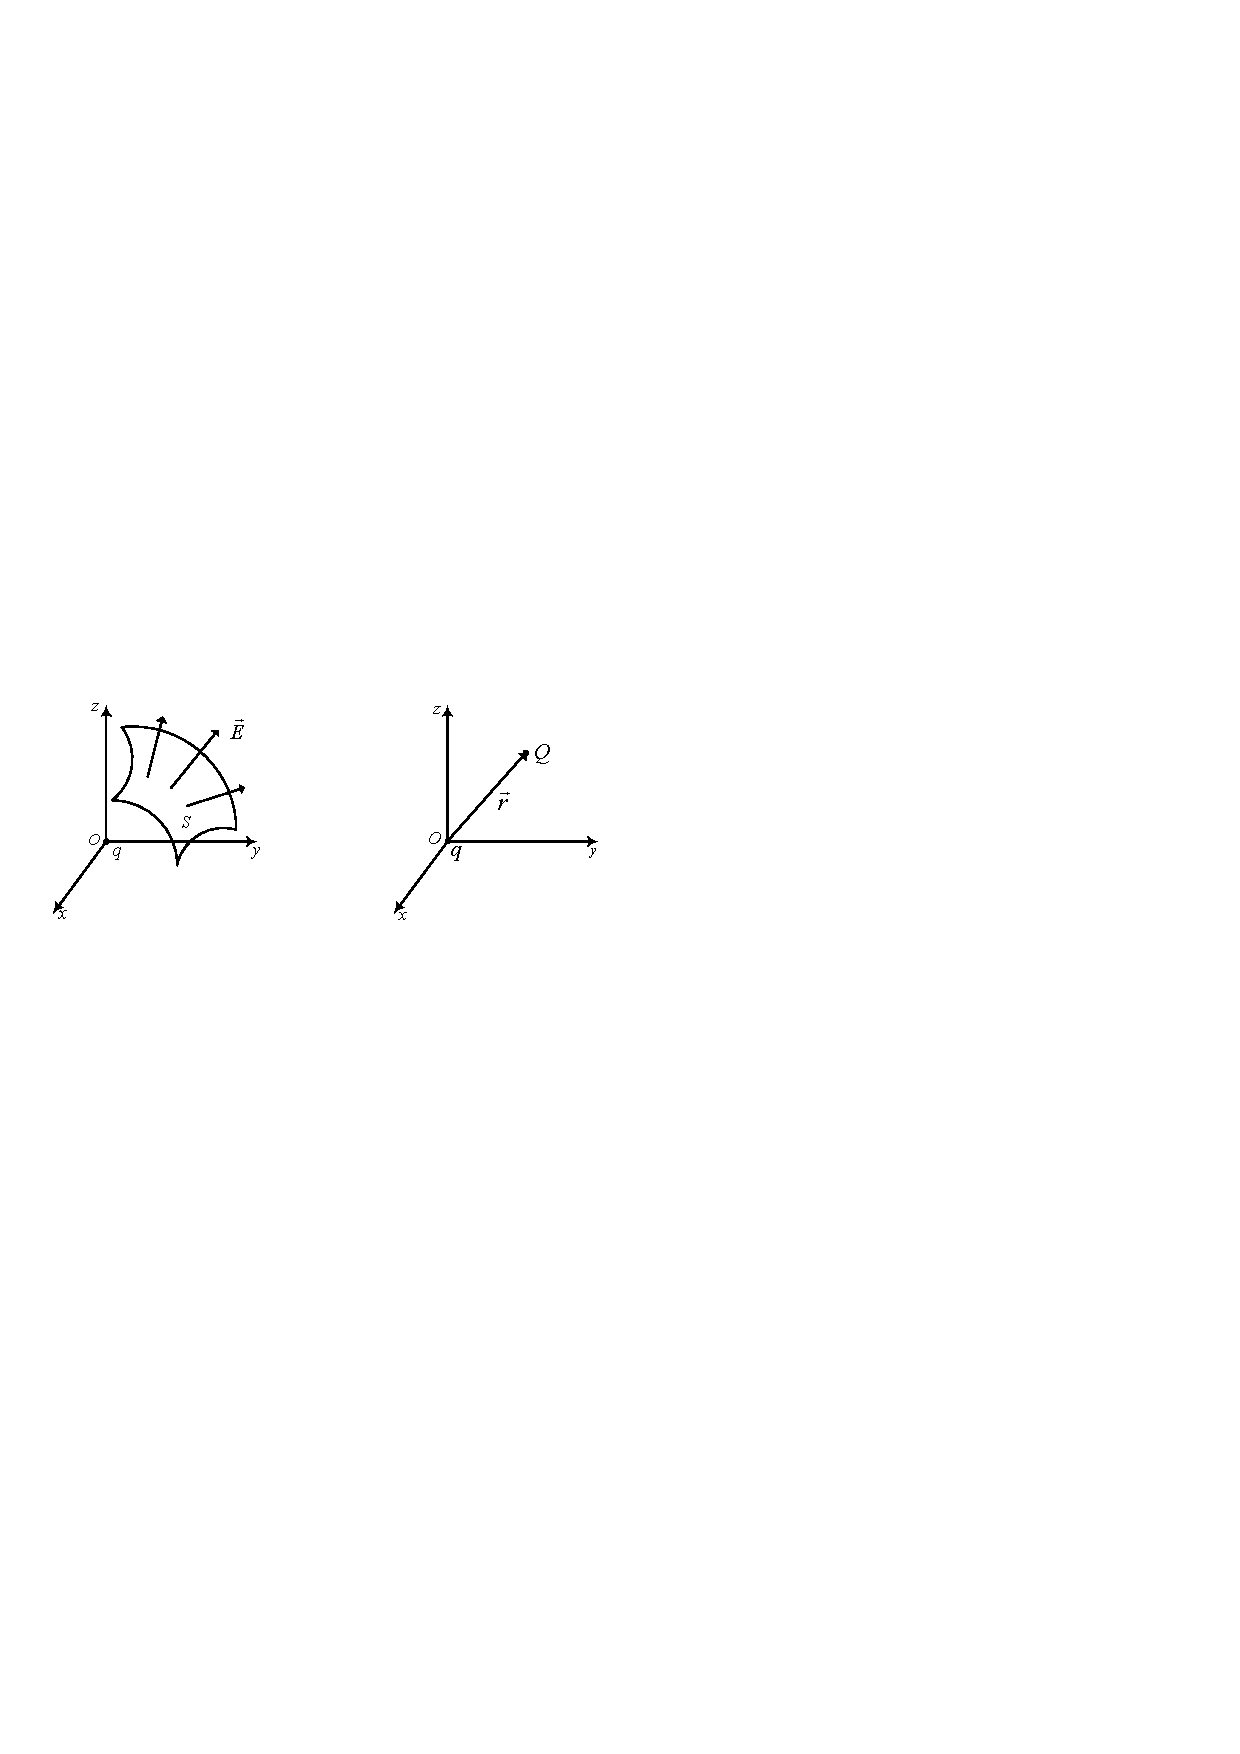
\includegraphics[width=0.8\textwidth]{Figures/EandCoulumb}
	\caption {左:穿过曲面$S$的电通量示意图,右:试探电荷$Q$在$\bm{r}$处所受库仑力示意图. }
	\label{eandcoulumb}
\end{figure}

\paragraph{电场在真空中的高斯定律}








\section{电磁场的势表示}
\section{电磁波及其在空间中传播的模型}
\section{无界区域的处理 —— 吸收人工边界方法}






\end{document}













